\section{Methodology}

\subsection{Problem Setup}

The definition of implicit sentiment in different research work \cite{PanDongXing2020,samuel2022direct,wang2020chinese} are slightly different. This paper integrates the expressions of the definitions, and defines implicit sentiment as: ``a fragment of language that does not directly contain obvious sentiment cues but expresses subjective sentiment", where ``fragment of language" includes words, phrases and sentences, and does not include a paragraph composed of several sentences. On this basis, this paper defines implicit sentiment analysis task as the task of ``sentiment analysis of Chinese implicit sentiment utterances that do not contain obvious sentiment words", and further abstracts it into a triple classification task, which classifies the possible sentiment tendencies of the sentences to be analyzed into `Positive', `Neutral', `Negative'.

The implicit sentiment analysis task is defined formally as follows: for any implicit sentiment sentence $ s = \{w_1,w_2,\dots,w_N\}$ and its context input to the model, output the model's prediction $P_t$ of sentence $s$ , and the Eq.~\ref{formula:classification-definition}~ defines the Chinese implicit sentiment sentence classification task.

\begin{equation}
    f(s) \rightarrow P_t=\left\{p_{t_0}, p_{t_1}, p_{t_2}\right\}\label{formula:classification-definition}
\end{equation}

where $N$ is the number of words contained in a given sentiment sentence, $w_n$ is the $n$th word in the sentence, $ n \in N $; $p_t$ is the probability that the implicit sentiment sentence $s$ belongs to a category, $p_{t_0}$ denotes the probability that the implicit sentiment sentence is neutral, $p_{t_1}$ denotes the probability that the implicit sentiment sentence is positive, $p_{t_2 }$ denotes the probability that the implicit sentiment sentence is negative.

\subsection{Knowledge Graph And Knowledge Retrieval}

Due to the lack of explicit sentiment words in implicit sentiment sentences, continuing to dig deeper into the semantic information latent in the text itself does not provide more adequate sentiment clues.
At this point, it is possible to associate the process of solving the problem with the human brain, which is to draw on rich external background knowledge.
Specifically, additional knowledge information can be introduced from the existing common sense knowledge graphs as sentiment cues for implicit sentiment analysis.

ConceptNet \footnote{https://conceptnet.io/} is a comprehensive commonsense knowledge graph, which is essentially a large semantic network describing concepts such as words and phrases that people use and the commonsense relationships between them, covering spatial, physical, social, temporal, and psychological aspects of everyday life.
ATOMIC \cite{sap2019atomic} is an event-centric knowledge graph. Recently, based on ATOMIC, Li et al. \cite{li2022c3kg} proposed a Chinese Commonsense Conversation Knowledge Graph (C3KG), which incorporates both social commonsense knowledge and dialog flow information, and is an important complement to Chinese common sense knowledge sources.

However, it is inefficient and unwise to retrieve sentiment knowledge triples directly in these huge knowledge bases which are oriented to almost all domains. Therefore, in this paper, a three-step triple extraction method is designed to extract valuable knowledge triples for the target implicit sentiment sentences.


\paragraph{Knowledge triples extraction based on rules}

The latest ConceptNet 5.5 includes a total of 34 different kinds of relations, and C3KG is divided into four main relationship patterns. The number of knowledge triples varies greatly across relationship types.
After analyzing the knowledge triples in the Chinese part of ConceptNet5, we found that the top 5 types of relationships account for more than 60\% of all relationships, including ``Synonym", ``RelatedTo", ``Causes", ``ExternalURL", and ``MotivatedByGoal''.
By observing the specific triple examples in ConceptNet5, it was obtained that the relations with the highest number of relations ``Synonym", ``RelatedTo" and others such as ``AtLocation'' have almost the same semantics between their corresponding head entity and tail entity or do not effectively provide additional sentiment cues, which leads to such relations being useless for sentiment analysis tasks. Instead, the model performance is greatly degraded by the large number of irrelevant knowledge retrieval processes and the introduction of redundant knowledge.
Similarly, for C3KG, it is observed that ``Emotion Cause Flow'', among the four relational models, has the greatest potential for implicit sentiment analysis tasks, while the other three relational models, ``emotion Intention Flow'', ``event flow'', and ``concept flow'', can only extend semantic information at the factual level, but do not introduce sentiment cues well.
Therefore, for the knowledge triple $t_k = (h, r, t) \in T$ (where $h$ and $t$ represent the head entity and tail entity, respectively, and $r$ denotes the relationship between two entities), the knowledge triples with these relationship types are firstly eliminated from the common knowledge base, which means only the triples with $ r \in R $ are retained, and $R$ denotes the set of valid relationships only after filtering.

Furthermore, in order to be able to introduce additional sentiment cues from the external knowledge graph efficiently, it is agreed that only one of the two, head entity $h$ and tail entity $t$, exists in the target implicit sentiment sentence $s \in C$.
With the above two rule constraints, it is possible to filter out those knowledge triples that introduce knowledge into the target implicit sentiment sentence.

\paragraph{Knowledge triples extraction based on sentiment dictionary matching}


After the rule-based knowledge triples extraction, in order to further extract the knowledge triples valuable for the implicit sentiment analysis task from the knowledge graph, explicit sentiment clues need to be introduced.
For the knowledge triple $t_k = (h, r, t) \in T$, $ h \in s $ or $ t \in s $, the entity not in the target implicit sentiment sentence is matched using the sentiment dictionary $d$, which is the concatenation of the three mainstream Chinese sentiment dictionaries. Knowledge triples without explicit sentiment cue words were subsequently eliminated.
After such matching and filtering, those sentiment knowledge triples with only one entity as an explicit sentiment word were selected to ensure that additional sentiment information could be introduced into the target implicit sentiment expression sentences.

\paragraph{Knowledge triples extraction based on event matching}

The sentiment knowledge triplets filtered by the above two filtering methods match the content of the target sentence at the character level. In order to be able to draw more fully on the relationship between events and sentiments embedded in the knowledge base, it is also necessary to extract sentiment events in the target sentences.

Sentiment expressions contain many colloquial expressions and complex sentence structures. In order to effectively extract sentiment events from the target implicit sentiment sentences, we adopt the same method for event extraction as that worked in the literature, and achieve effective extraction of sentiment events from the target implicit sentiment sentences through the methods and steps of Pre-processing, Verb-driven, Adjective-driven, and Recursive Applying.
For example, for the implicit sentiment expression ``Probably got a cold and stay up late, it is still some pain'', the sentiment event ``somebody gets cold'' can be extracted, which corresponds to the C3KG and can be associated to the sentiment triple $(personX\ gets\ cold, xAttr, Uncomfortable)$, and ``Uncomfortable'' is a negative sentiment tendency in the sentiment dictionary, thus introducing explicit sentiment cues.

Finally, since ConceptNet and C3KG are multilingual general knowledge base, although it contains some knowledge triples in Chinese, it is still more based on entity relationship pairs in English or other languages. For this reason, the knowledge in those knowledge bases are translated into Chinese as well as aligned and merged with the Chinese part through online translation. The merged knowledge graph is finally used as the main source of external knowledge in this paper.

\subsection{Sentiment Analysis Incorporating Contextual Information And External Common Sense Knowledge}

This method adaptively fuses knowledge from external common sense knowledge graphs by designing knowledge retrieval mechanisms in this paper in the process of learning textual representations.
By doing so, a process similar to that of the human brain in understanding implicit emotional expressions is simulated, i.e., drawing on one's own experience or common sense to distinguish sentiment tendencies, allowing the model to achieve a deeper understanding of the text beyond the literal semantic information.

The above model network framework diagram is shown in Fig~\ref{fig:framework-of-the-model}~. The model consists of four layers: input layer, adaptive knowledge fusion layer, multipolar attention layer fusing contextual contexts, and output layer. The structure of each layer is described in detail in the following.

\begin{figure}[h]
    \centering
    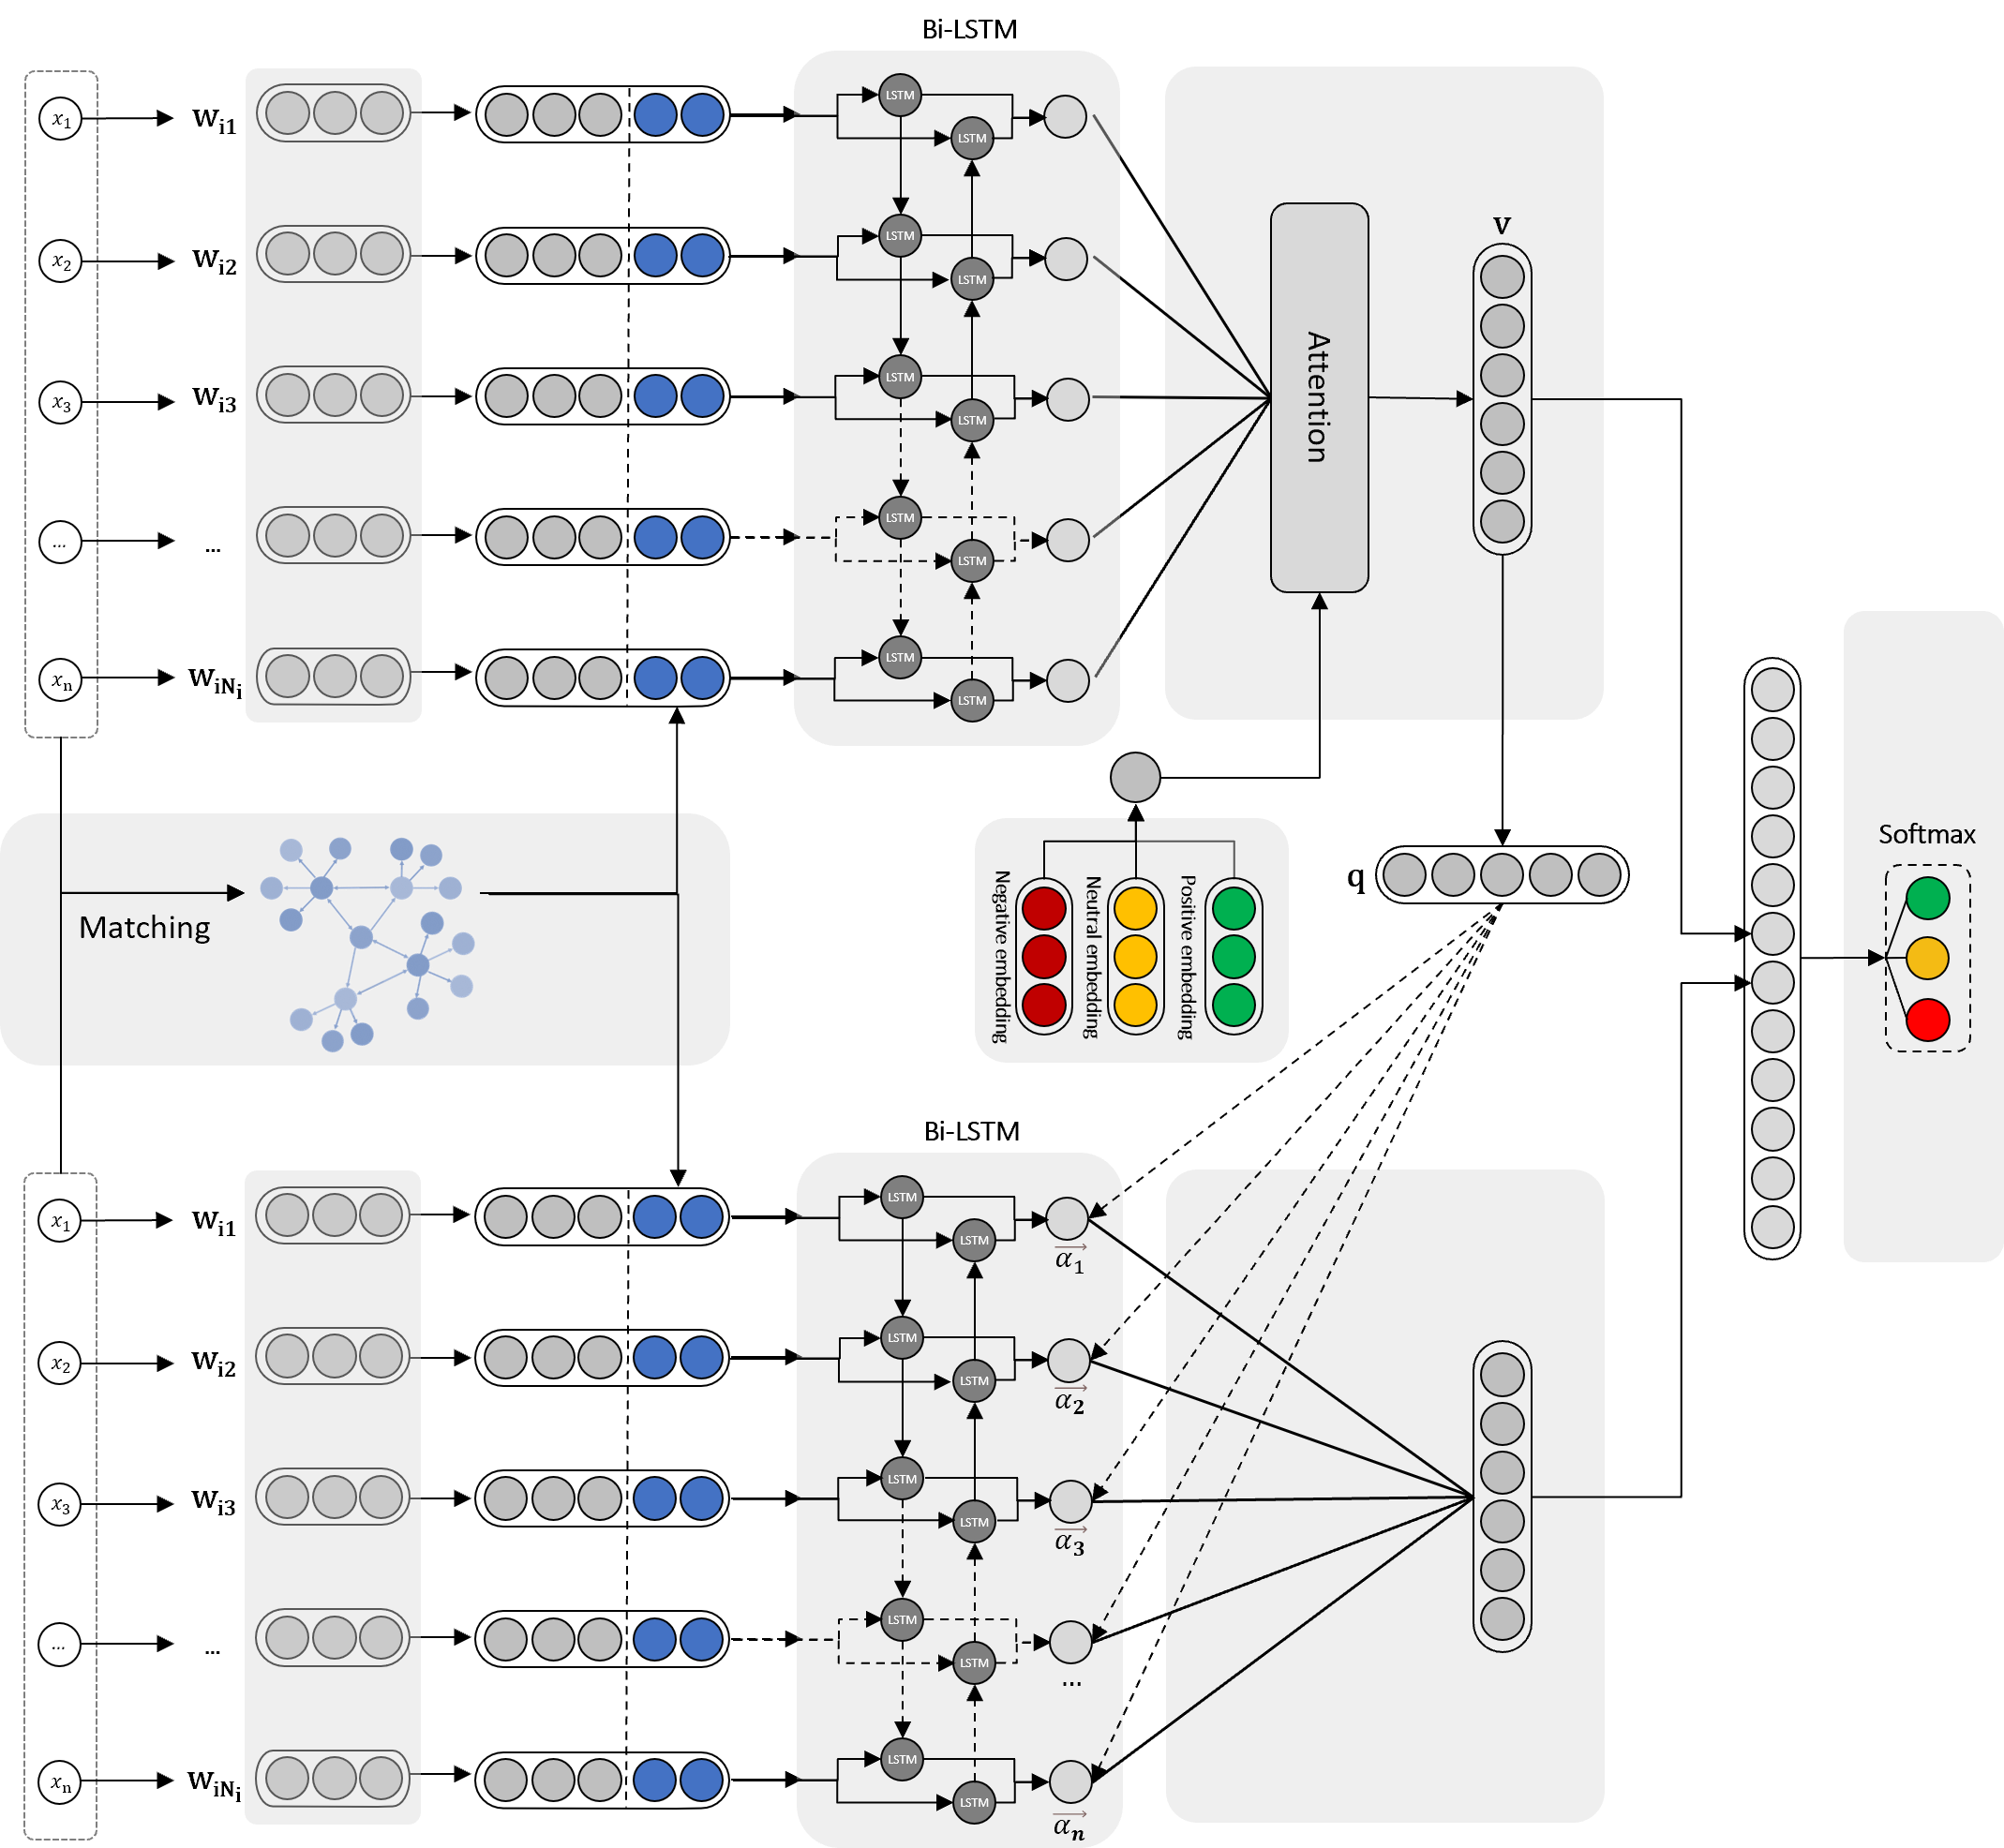
\includegraphics[width=0.8\linewidth]{submissions/knowledge-sentiment-analysis/1.png}
    \caption{Framework of the model}
    \label{fig:framework-of-the-model}
\end{figure}

\paragraph{Input layer}
For the input of the pre-trained model, the implicit sentiment text needs to be encoded first. For the original corpus input, each word or phrase ${x_i}$ in the sentence is hard-coded into the corresponding vector representation by one-hot encoding representation.
The pretrained model uses Transformer as its feature extractor, and also needs to encode the word-by-word position information in the text to obtain the word position representation vector. Finally, the above vector representations are combined and input to the pretrained model to obtain the continuous word embeddings $\vec{w}_{t} \in R^{d_{e}}$ encoded with contextual information, which are used as input information for the next layer.

\paragraph{Adaptive knowledge fusion layer}

In order to better fuse the extracted sentiment knowledge triples with the target implicit sentiment sentence information, a knowledge fusion strategy is needed. For each target implicit sentiment sentence $s$, more than one sentiment knowledge triple may be extracted, i.e., the set of triplets $G=\left\{g_{1}, g_{2}, \ldots, g_{n}\right\}$ can be obtained.
The set of knowledge triplets $G$ extracted from it is regarded as a knowledge graph $G^{i}=\left\{g_{1}^{i}, g_{2}^{i}, \ldots, g_{n}^{i}\right\}$. Using the TranR model \cite{lin2015learning} for each knowledge triple $ g_{j}^{i}=\left(h_{j}, r_{j}, t_{j}\right)$ in $G^{i}$, we obtain the knowledge embedding representation $\boldsymbol{g}_{j}^{i}=\left(\boldsymbol{h}_{j}, \boldsymbol{r}_{j}, \boldsymbol{t}_{j}\right)$. The head entity $h$ is designated as the entity in the target implicit sentiment sentence, and the tail entity $t$ is the entity in the external sentiment knowledge graph.
Using the representations of all head and tail entities learned in the knowledge graph $G^{i}$ in the knowledge subgraphs, their weights are calculated adaptively by the attention mechanism, and the embedded representations of the knowledge subgraphs are learned by this to represent the sentiment cues introduced for the target implicit sentiment sentence, calculated as shown in the Equ.~(\ref{formula_4_1}).
\begin{equation}
    \boldsymbol{G}^{i}=\sum_{j=1}^{n} (\operatorname{softmax}(\boldsymbol{W}_{tv} \boldsymbol{t}_{j}\frac{\boldsymbol{t}_{j}^{T}\boldsymbol{W}_{tk}^{T}\boldsymbol{W}_{h} \boldsymbol{h}_{j}}{\sqrt{d}})+\boldsymbol{W}_{r} \boldsymbol{r}_{j})\label{formula_4_1}
\end{equation}

where $\boldsymbol{W}_{h}, \boldsymbol{W}_{tk},\boldsymbol{W}_{tv}, \boldsymbol{W}_{r} \in \mathbb{R}^{l \times m}$ are the parameter matrices of head entities, tail entities and relations. $\boldsymbol{h}_j, \boldsymbol{t}_j, \boldsymbol{r}_j \in \mathbb{R}^m$.

The knowledge graph embedding representation $\boldsymbol{G}^i$ obtained by learning represents the additional external common knowledge introduced, and if the target sentiment sentence cannot be matched to any sentiment knowledge triplet, $\boldsymbol{G}^i$ is treated as a zero vector.
The word embedding $\boldsymbol{w}_{i}$ obtained in the ``input layer" is fused with $\boldsymbol{G}^i$ to achieve the introduction of external common sense knowledge, and finally the result $\boldsymbol{e}_i=\boldsymbol{ w}_i \oplus \boldsymbol{G}^i$ is input to the next layer.

\paragraph{Multipolar attention layer fusing contextual contexts}

This layer models the fusion of implicit sentiment expressions and contextual information using multipolar attention mechanisms to extend the information in implicit sentiment expressions.

As for the text implicit sentiment classification task, the output of the current moment is not only related to the state before the current moment, but may also related to the state after the current moment.
In this layer, the input of the upper layer network first passes through a bi-directional long and short-term memory network (Bi-LSTM), Bi-LSTM is composed of an LSTM with forward processing sequences and an LSTM with reverse processing sequences, considering both forward and backward sequences, making full use of contextual information and allowing deep feature extraction of the contextual information inside the input sentence.

As mentioned in the literature \cite{wei2020BiLSTM}, the difference between attention weights for specific polarities is an important feature of the Chinese implicit sentiment analysis task.
Therefore, multi-polar attention mechanisms are introduced in this layer to incorporate sentiment polarity labeling information into the implicit sentiment representation. Specifically, polarity-specific queries are introduced by using attention mechanisms with different polarities in order to make the attention mechanism more focused on the differences between different sentiment polarities.The calculation formula are shown in Eq.~(\ref{formula_4_2}), Eq.~(\ref{formula_4_3}), Eq.~(\ref{formula_4_4}).

\begin{equation}
    \boldsymbol{v}^q=\sum_{i=1}^T \alpha_i^q \boldsymbol{t}_i
    \label{formula_4_2}
\end{equation}

\begin{equation}
    \alpha_i^q=\frac{\exp \left(e_i^q\right)}{\sum_{k=1}^T \exp \left(e_k^q\right)}
    \label{formula_4_3}
\end{equation}


\begin{equation}
    e_i^q=\boldsymbol{q} \boldsymbol{W} \boldsymbol{m}_i
    \label{formula_4_4}
\end{equation}

where $ \boldsymbol{v}^q $ represents the embedding representation of sentences under sentiment polarity $q$. $T$ is the length of the target implicit sentiment sentence.$ \alpha_i$ is the normalized weight of the word or character $w_i$ computed from the Bi-LSTM output $ \boldsymbol{t}_i $. $ e^q_i$ is the attention score of $w_i$. The matrix $\boldsymbol{W}$ is then used to query the weight matrix of $q$ and $\boldsymbol{h}_i$ in the bilinear function. $\boldsymbol{q} \in \boldsymbol{Q}=\left\{\boldsymbol{q}_{\text{pos}}, \boldsymbol{q}_{\text{neg}}, \boldsymbol{q}_{\text{neu}}\right\}$ correspond to polarity-specific query embedding representations of positive, negative and neutral sentiment polarity, respectively. The same sentiment dictionary as in the knowledge triad extraction process above is used here to initialize the polarity query embedding representation, which is computed by averaging the embeddings of sentiment words with the same sentiment polarity in the sentiment dictionary, as shown in Eq.~(\ref{formula_4_5}):

\begin{equation}
    \boldsymbol{q}=\frac{1}{N} \sum_{i=1}^N \boldsymbol{w}_i^q
    \label{formula_4_5}
\end{equation}


$\boldsymbol{w}_i^q$ is a pre-trained embedding representation of the word or character $w_i$ whose sentiment polarity belongs to $q$, $q \in Q=\left\{q_{\text {pos }}, q_{\text {neg }}, q_{\text {neu }}\right\}$.

The implicit sentiment sentence representations with weights under the three sentiment polarities are spliced to obtain a new representation of the implicit sentiment expression $\boldsymbol{v}=\boldsymbol{v}^{q_{pos}} \oplus \boldsymbol{v}^{q_{neg}} \oplus \boldsymbol{v}^{q_{neu}}$.


The context representation is considered as a whole, and the implicit sentiment sentence representation $q^c$ transformed by the fully connected layer is used as the query vector to assign weights to each word in $C$ in order to achieve the extraction of key features in the contextual information of the target implicit sentiment expression by the model through the attention mechanism.


\begin{equation}
    \boldsymbol{v^c}=\sum_{i=1}^{T_C} \alpha_j^c \boldsymbol{t}_i
    \label{formula_4_6}
\end{equation}

\begin{equation}
    \alpha_j^c=\frac{\exp \left(e_j^c\right)}{\sum_{k=1}^m \exp \left(e_k^c\right)},
    \label{formula_4_7}
\end{equation}

\begin{equation}
    e_j^c=\boldsymbol{q}^c \boldsymbol{W}^c \boldsymbol{h}_j^c
    \label{formula_4_8}
\end{equation}

\begin{equation}
    \boldsymbol{q}^c=\tanh (\boldsymbol{W} \boldsymbol{v}+\boldsymbol{b})
    \label{formula_4_9}
\end{equation}

Finally, by splicing the implicit sentiment sentence representation $\boldsymbol{v}$ with the contextual representation $\boldsymbol{v^c}$, the implicit sentiment sentence representation $\boldsymbol{v_{out}}$, which incorporates the contextual information, is obtained as the output of this layer, and it is fed into the output layer for the final probability calculation, as shown in Equ.~(\ref{formula_4_10}):
\begin{equation}
    \boldsymbol{v_{out}}=\boldsymbol{v} \oplus \boldsymbol{v^c}
    \label{formula_4_10}
\end{equation}

\paragraph{Output layer}

In the output layer, an implicit sentiment sentence representation $\boldsymbol{v_{out}}$ incorporating contextual information is projected into the sentiment polarity category space using a fully connected network. Then, the scores of each category are normalized to an approximate probability value $\widehat{\boldsymbol{y}}$ by the calculation of the Eq.~(\ref{formula_4_11}).
\begin{equation}
    \widehat{\boldsymbol{y}}=\operatorname{softmax}\left(\boldsymbol{W}_{\text {out }} \boldsymbol{v}^{\mathrm{T}}+\boldsymbol{b}_{\text {out }}\right)
    \label{formula_4_11}
\end{equation}
where $\boldsymbol{W}_{\text{out}}$ and $\boldsymbol{b}_{\text{out}}$ are the weight matrix and bias, respectively.
